\ylDisplay
{a}% Problem name
{2021}% Year
{mcq}% Round (mcq, theory, experiment)
{3}% Problem nr.
{physics}% Subject (physics, chemistry, biology)
{}% Difficulty (1-3)
{
% Syl:
\ifStatement
In the following circuit, the current through the resistor $R_1=(\SI{2}{\ohm}$ is
\begin{center}
  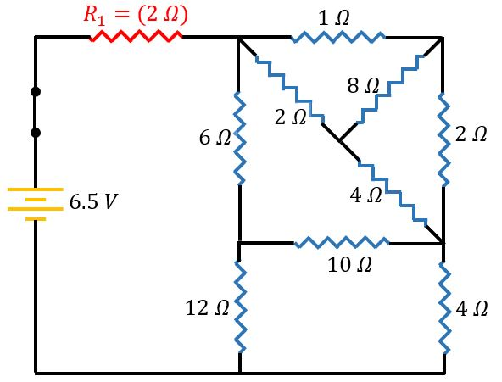
\includegraphics[width=0.5\linewidth]{2021-mcq-03-p}
\end{center}
\fi


\ifOption1
\SI{0.5}{\A}
\fi


\ifOption2
\SI{1.0}{\A}
\fi


\ifOption3
\SI{1.8}{\A}
\fi


\ifOption4
\SI{2.0}{\A}
\fi


\ifHint

\fi


\ifSolution

\fi


\ifEstStatement
% Problem name:

\fi


\ifEstOption1

\fi


\ifEstOption2

\fi


\ifEstOption3

\fi


\ifEstOption4

\fi


\ifEstHint

\fi


\ifEstSolution

\fi
}
